\documentclass[10pt, a4paper]{beamer}

\usetheme{Berkeley}
\usecolortheme{sidebartab}

\documentclass{article}
\usepackage{graphicx}

\begin{document}
	\setbeamertemplate{sidebar left}{}
	\title{Progress Presentation-I}
	\subtitle{e-Yantra Summer Intership-2016 \\ $Autonomous-Drone$}
	\author{Akshit Gandhi\\Keyur Rakholiya\\
	Mentors:\\ Pushkar Raj\\Akshat Jain\\Rama Kumar}
	\institute{IIT Bombay}
	\date{\today}
	%\addtobeamertemplate{sidebar left}{}{\includegraphics[scale = 0.3]{logowithtext.png}}
	\frame{\titlepage}

\setbeamertemplate{sidebar left}[sidebar theme]
\section{Overview of Project}
\begin{frame}{Overview of Project}
	\textbf{Autonomous-Drone} \\
	\begin{itemize}
		\item Objective:\\
		            “Making an Autonomous Drone that can travel from one point to another based on its GPS Location. This drone can be used for tracking objects and aerial photography when interfaced with an Object Tracking Camera system.”

		\item Deliverables:\\
	1. An Autonomous Drone\\
2. Code and Documentation\\
3.Tutorials explaining individual modules

	\end{itemize}
\end{frame}

\section{Overview of Task}
\begin{frame}{Overview of Task}
\textbf{Task list}
 	\hspace{0.45in}\\
 	\begin{tabular}{|c|c|}
 		\hline
 		Task & Deadline &
 		\hline
 		Calculations for making a Quadcopter & 3/6/16 &
 		\hline
 		Calibrating APM & 5/6/16 &
 		\hline
 		Assembling the quad for manual flight & 7/6/16 &
 		\hline
 		Interface Gps with APM & 9/6/16 &
 		\hline
 		Interface Raspberry-Pi with APM & 11/6/16 &
 		\hline
 		Manual flight using R-pi & 15/6/16 &
 		\hline
 		Auto take-off and land using R-pi & 19/6/16 &
 		\hline
 		Create a flight planning algorithm & 25/6/16 &
 		\hline
 		Autonomous Flight & 3/7/16 &
 		\hline
\end{tabular}
\end{frame}

\section{Task Accomplished}
\begin{frame}{Task Accomplished}
	\begin{itemize}
	    \item Research on drone project.
		\item Assembly of drone.
		\item Understanding software and Flight controller features.
		\item Interface GPS.
		\item TEST FLIGHT-1 done.
		\item Research on dronekit Library version.
		\item Installing Rasbarian linux on R pi.
		\item connect R-pi to Ardupilot via USART or USB
		\item Run python code on R pi to get data from Flight controller.
	\end{itemize}
\end{frame}

\begin{frame}{Images}
	Quadcopter with Mission planer software: \\
	\centering
		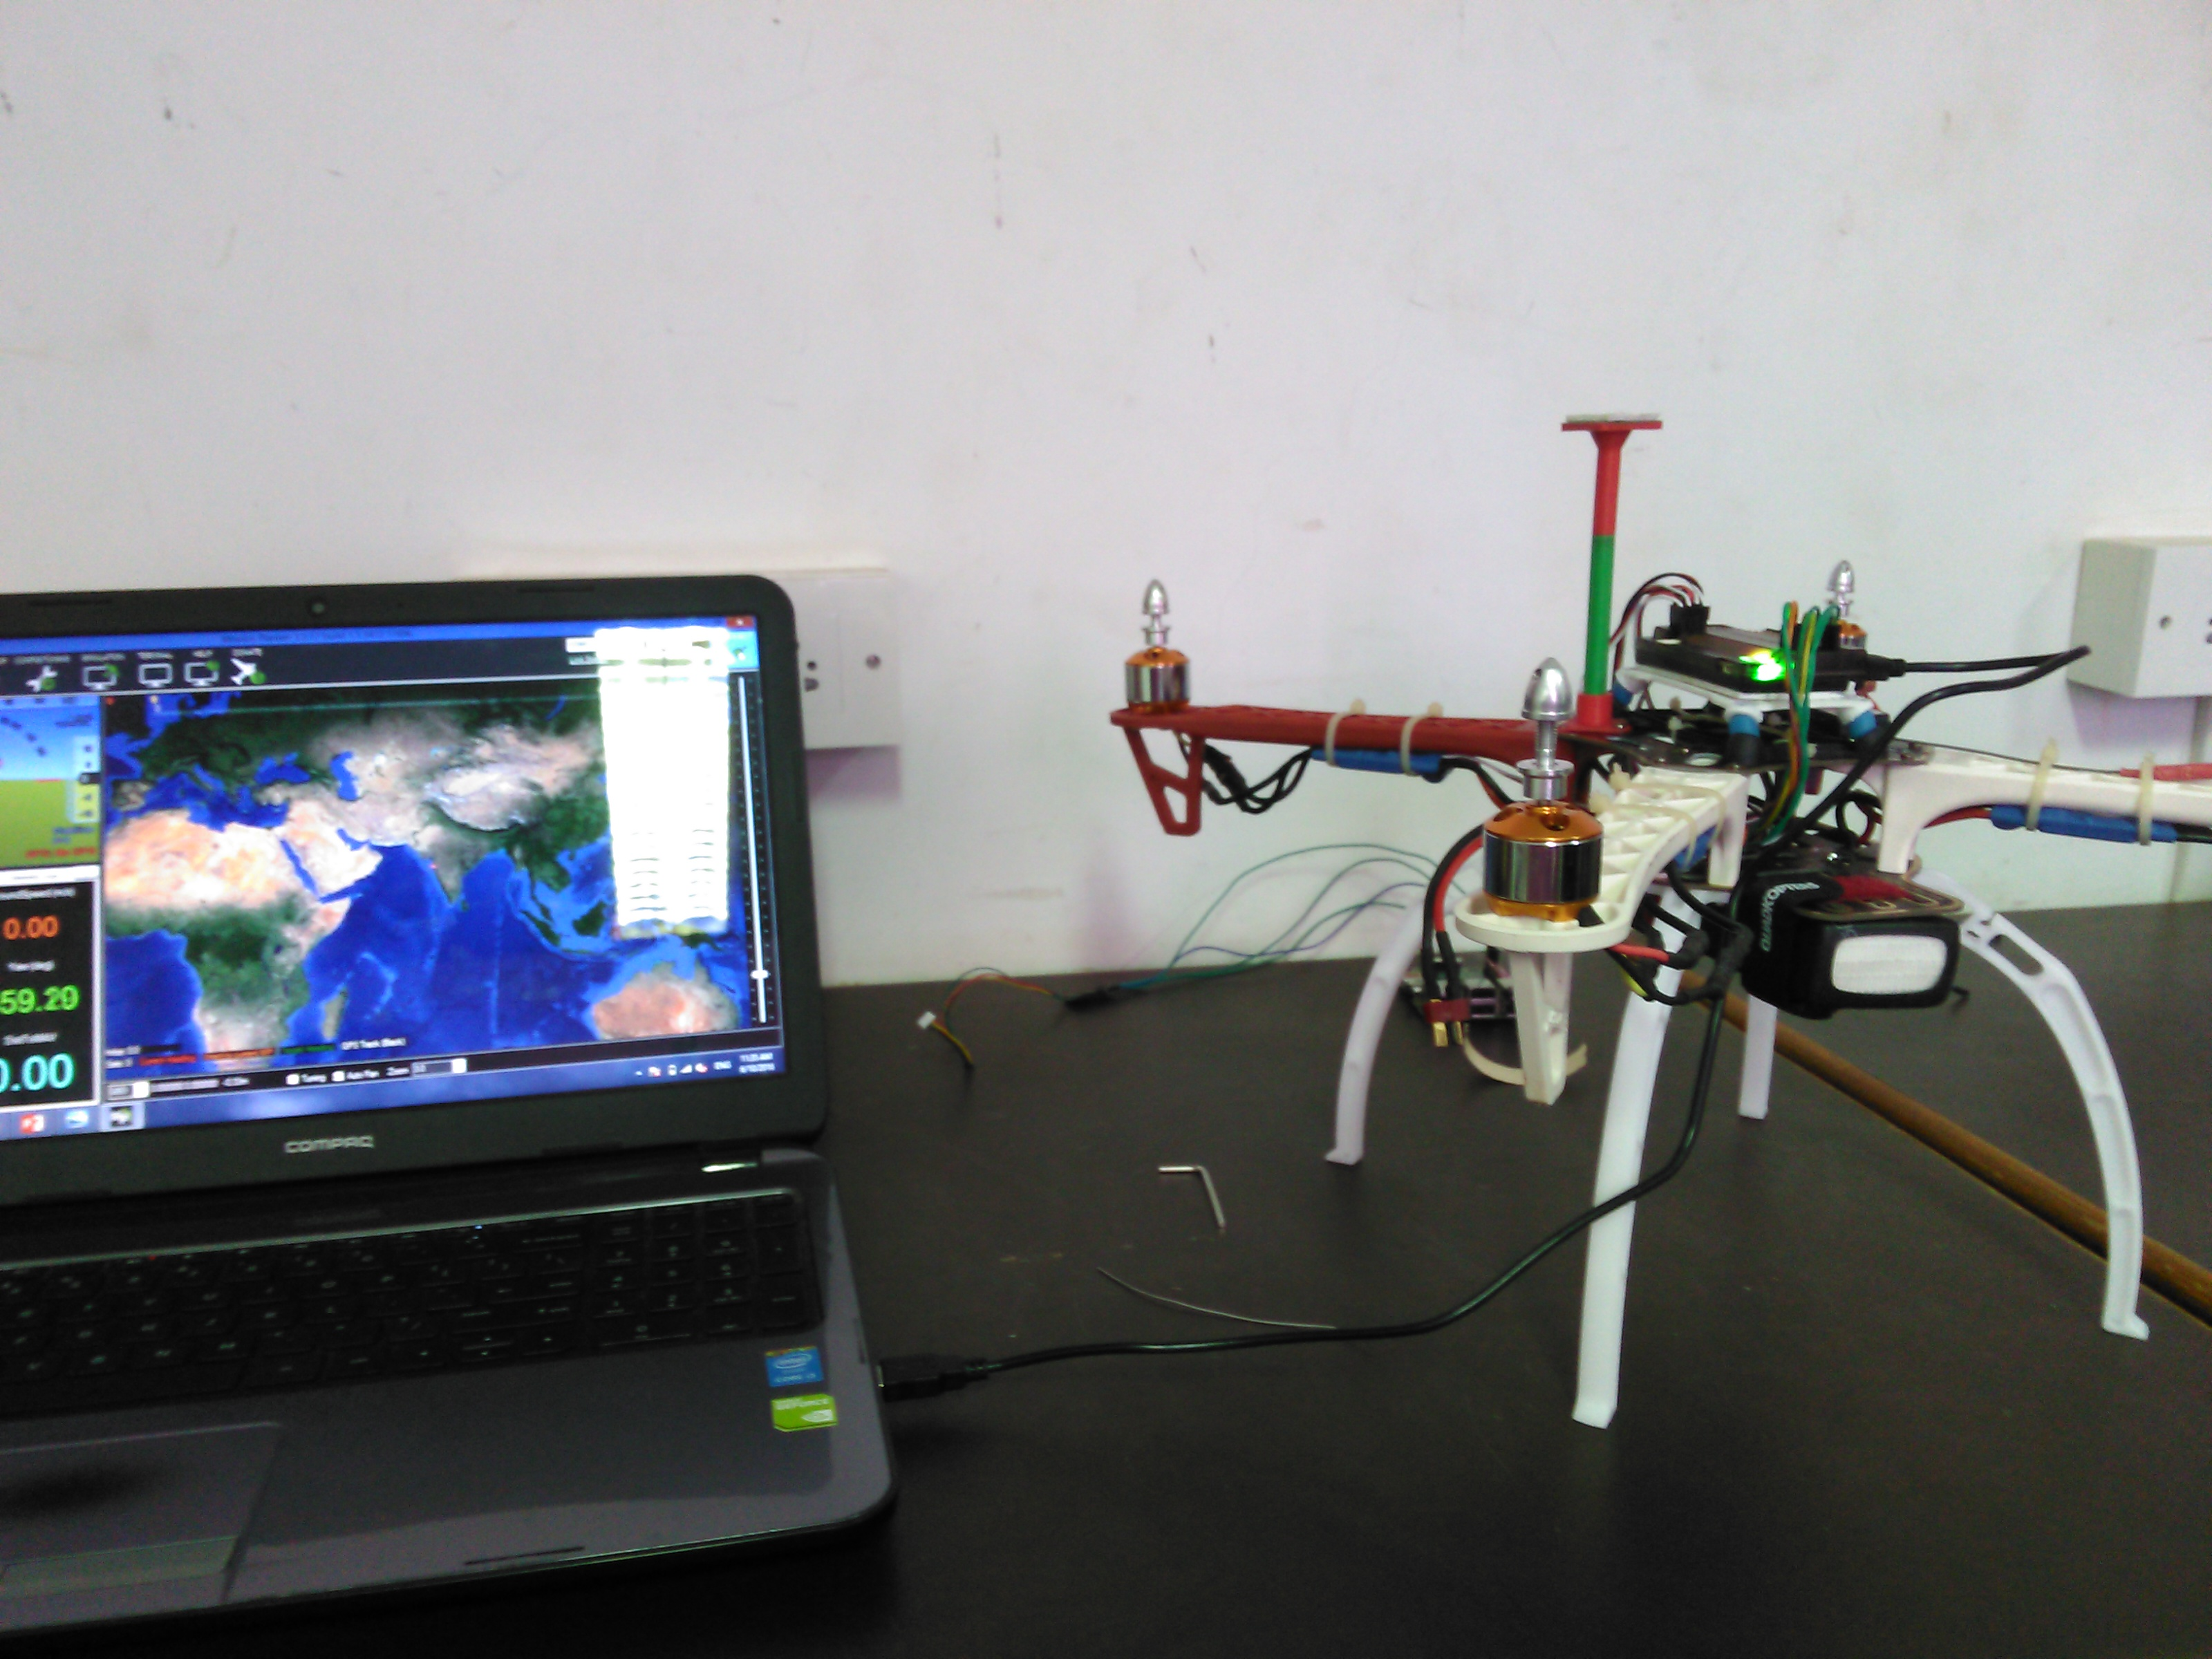
\includegraphics[width =200px]{qd1}

\end{frame}



\begin{frame}{Images}
	Ardupilot Flight Controller: \\
	    \centering
		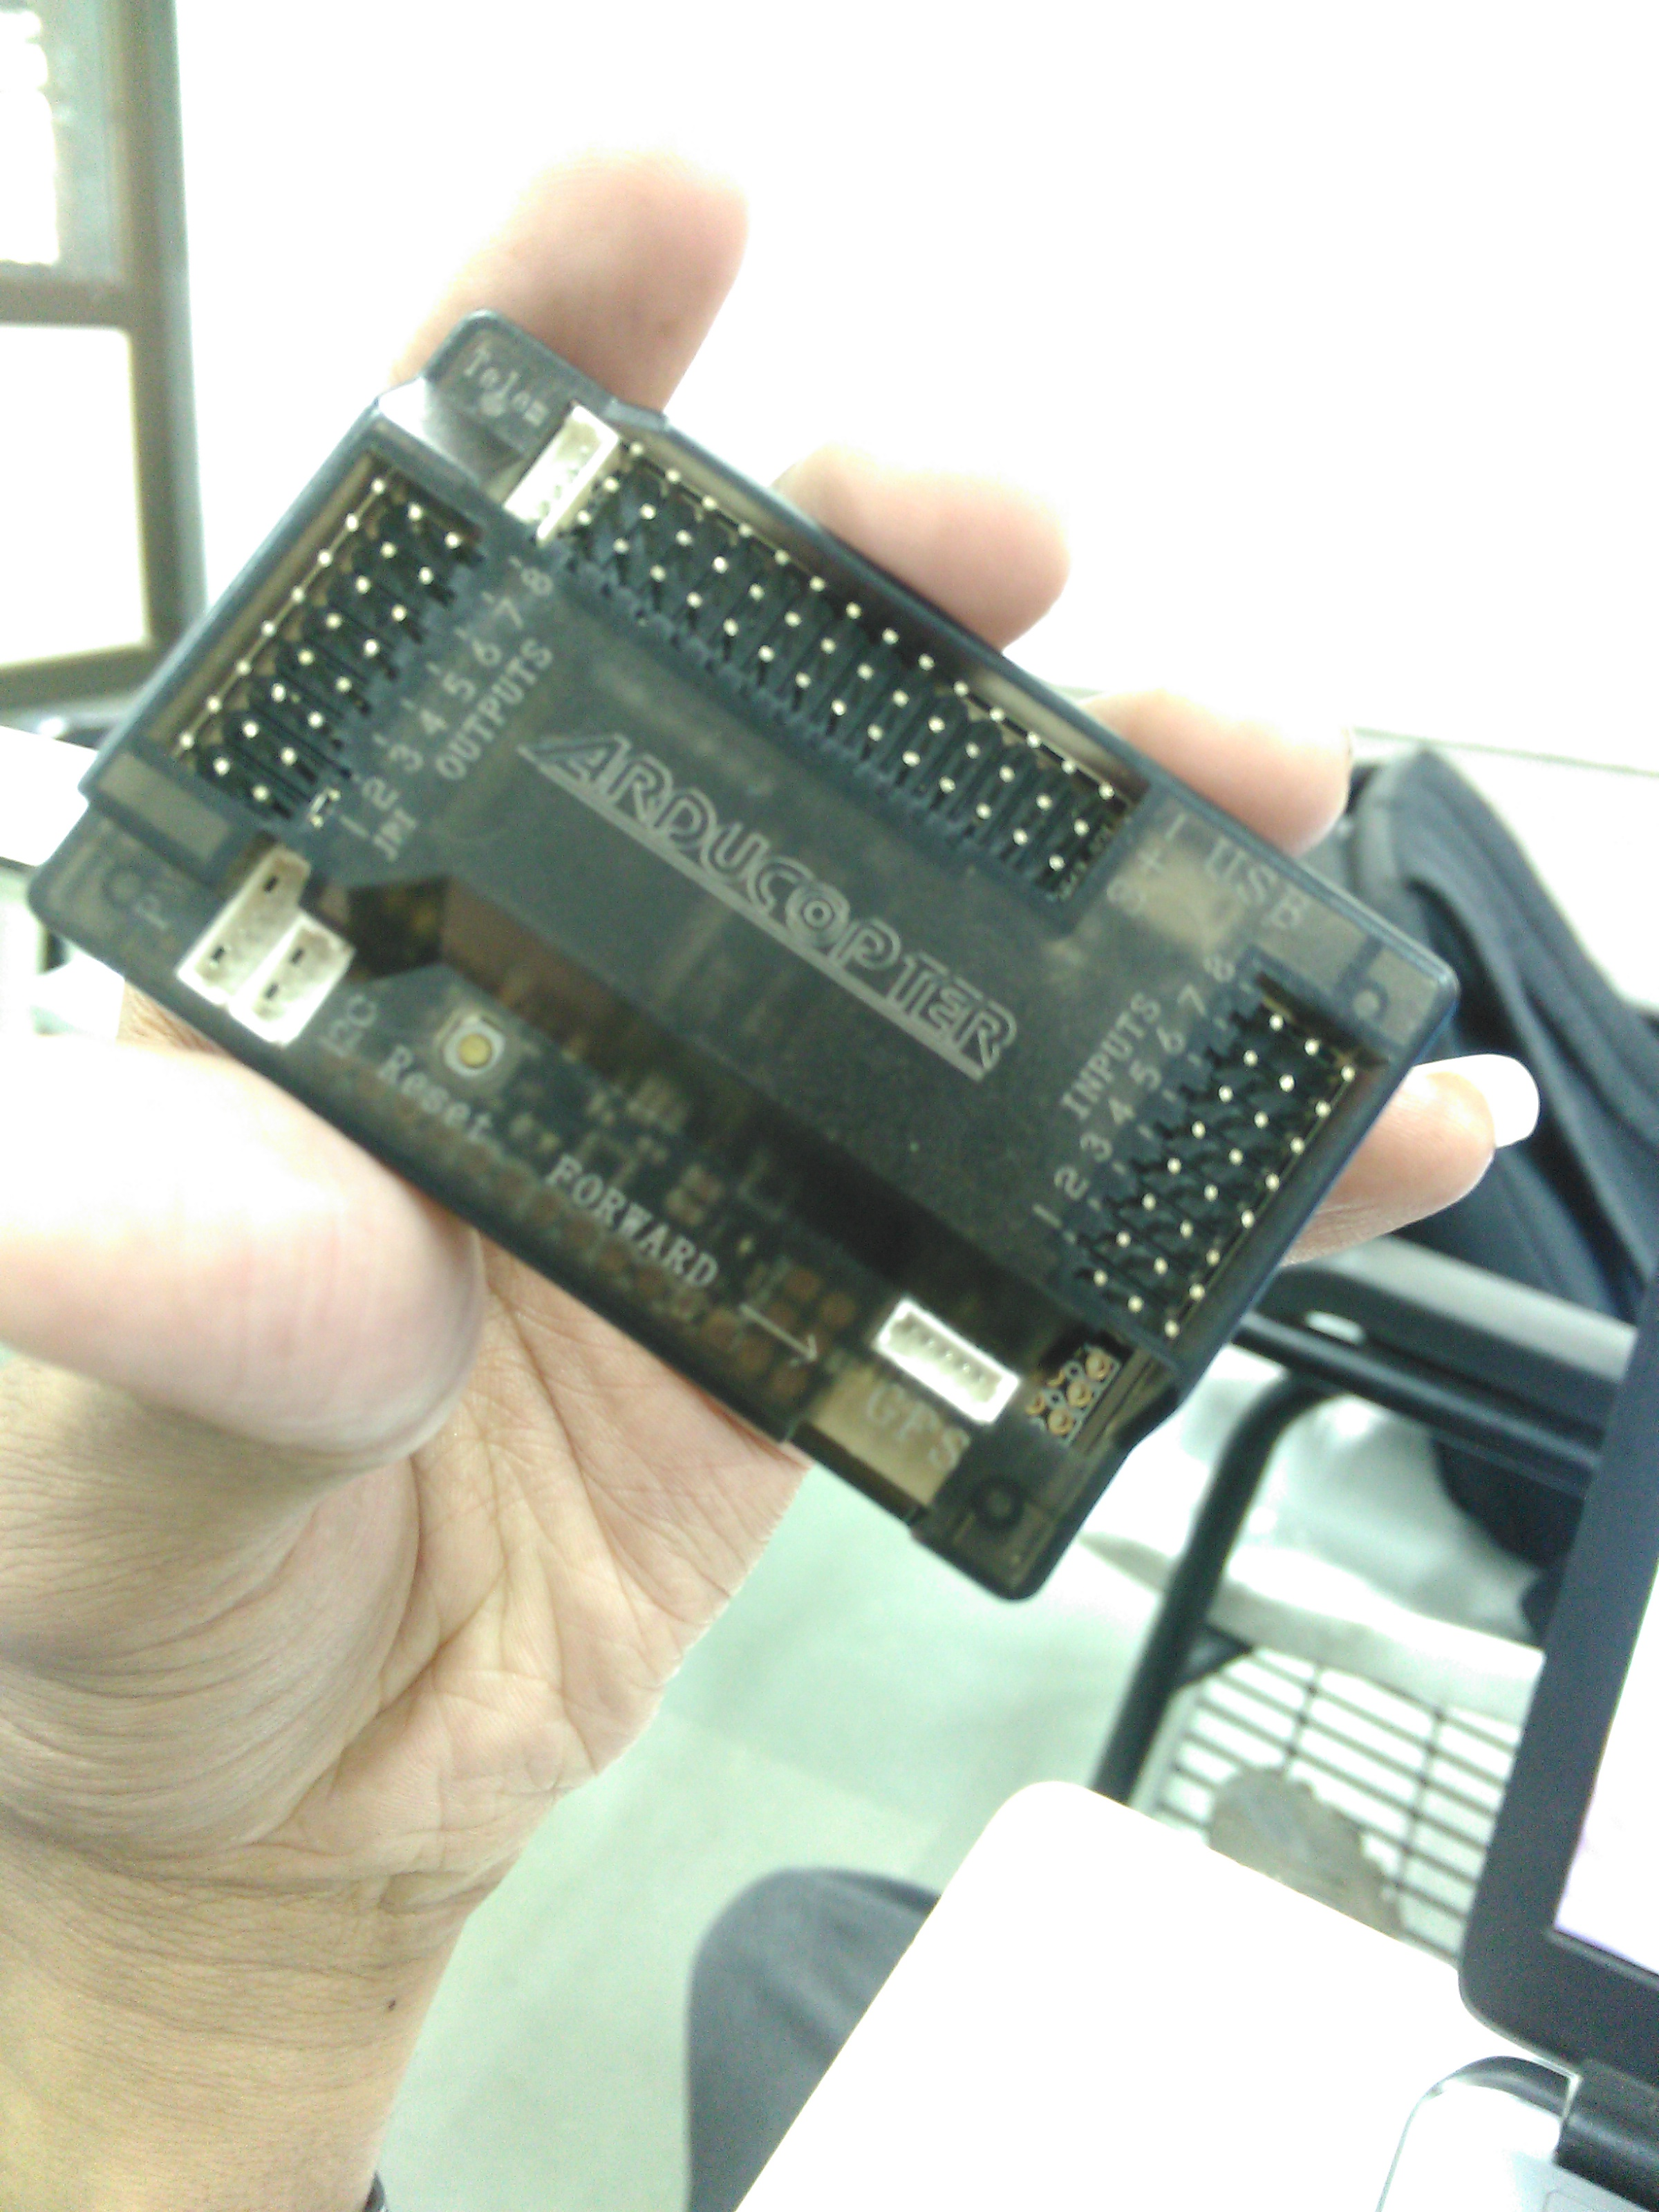
\includegraphics[width =200px]{fc}
\end{frame}


\section{Challenges Faced}
\begin{frame}{Challenges Faced}
     \large\textbf{Hardware challenges}
	\begin{itemize}
	    \item Calculation of total approx weight.
	    \item For lifting the drone, calculate the thrust
	    \item knowing the aerodynamics rules
	    \item Choose the right propellers in size and pitch
	    \item Calculate flight time
	    \item BLDC motor power rating and KVA rating
	    \item Choose right battery 
	    \item Carbon fiber frame for drone
	    \inem Interfacing sensors Like GPS,SONAR
	    
	\end{itemize}
\end{frame}

\section{Challenges Faced}
\begin{frame}{Challenges Faced}
     \large\textbf{Software challenges}
	\begin{itemize}
	    \item Ardupilot is open source Hardware.They release new version after fixing bugs! its very difficult to choose right firmware  for your hardware among hundreds of software
	    \item Finding out suitable version of MISSION PLANNER for your firmware
	    \item More then 239 parameters are there. according to our mission we have to make changes
		\item Calibration axis of gyro and radio channels.
	\end{itemize}
\end{frame}


\section{Future Plans}
\begin{frame}{Future Plans}
	\begin{itemize}
	    
		\item Writing code in python 
		\item Making drone autonomous\\
		By Autonomous, we mean that drone will fly and reach to our desire destination without Remote control.
		\item Mounting camera on drone , and making it object tracking drone
	\end{itemize}
\end{frame}


\section{Thank You}
\begin{frame}{Thank You}
	\centering THANK YOU !!!
\end{frame}
\end{document}
